%Dies ist die Vorlage für die einzelnen Kapitel, die jeweils mit Chapter als Kapiteltitel starten
\chapter{Kryptographie}
Die Kryptographie ist eine Wissenschaftslehre, die sich mit den Verfahren der Ver- und Entschlüsselung von Informationen sowie deren Anwendung befasst. Meistens werden dazu geheime Schlüssel oder Schlüsselpaare verwendet. Damit lassen sich mithilfe mathematischen Berechnungsverfahren, sogenannten Algorithmen, Nachrichten verschlüsseln. Heutige Verschlüsselungsverfahren basieren entweder auf einem symmetrischen oder asymmetrischen Algorithmus.

%mit \section{title} wird ein Unterkapitel der ersten Gliederungsebene überschrieben
\section{Grundlagen}


%mit \subsection{title} wird ein Unterkapitel der zweiten Gliederungsebene überschrieben
\subsection{Symmetrische Verschlüsselung}

Bei der symmetrischen Verschlüsselung wird sowohl zur Ver- und Entschlüsselung derselbe Schlüssel verwendet, der auch Shared Secret genannt wird. Mithilfe dieses Schlüssels und einem symmetrischen Verschlüsselungsalgorithmus wird die Nachricht des Absenders verschlüsselt. In diesem Zusammenhang wird der "lesbare Text einer Nachricht [...] Klartext [..] genannt" \footcite[S. 21]{Ertel2012}. Aus dem Shared Secret und dem Klartext wird durch eine mathematische Vorschrift ein Geheimtext erzeugt. Dieser verschlüsselte Text kann ausschließlich mit dem gleichen Schlüssel entschlüsselt werden, mit dem er verschlüsselt wurde.
Diese Tatsache wirkt sich im elektronischen Briefverkehr nachteilig auf die Anwendung der symmetrischen Verschlüsselung aus. Da beide Kommunikationspartner denselben Schlüssel benötigen, muss dieser zuvor ausgehandelt und übertragen werden. Die Übertragung dieses Schlüssels stellt ein Sicherheitsrisiko dar. Wird die Übertragung der Schlüssels abgehört, können Dritte mit seiner Hilfe die verschlüsselten Nachrichten mitlesen.

\subsection{Asymmetrische Verschlüsselung}

Wie bei der symmetrischen Verschlüsselung kommt auch bei der asymmetrischen Verschlüsselung, die auch Public-Key-Kryptography genannt wird, ein kryptographischer Algorithmus zum Einsatz. Hierbei wird jedoch wird statt eines gemeinsamen Schlüssels ein Schlüsselpaar verwendet. Dieser besteht aus einem öffentlichen und einem privaten Schlüssel, die mathematisch zusammenhängen. Jeder, der verschlüsselte Nachrichten empfangen möchte, verfügt über ein solches Schlüsselpaar. Der private Schlüssel wird niemals bekanntgegeben, wohingegen der öffentliche Schlüssel jedem zugänglich gemacht werden kann. Obwohl die Schlüsseln zusammenhängen, kann aus der Kenntnis des öffentlichen Schlüssels nicht auf den privaten Schlüssel geschlossen werden \footcite[S. 177]{Schmeh2013}.
Soll eine Nachricht durch ein asymmetrisches Verschlüsselungsverfahren verschlüsselt verschickt werden, wird zunächst der öffentliche Schlüssel des Empfängers benötigt. Zusammen mit der Nachricht wird der Geheimtext erzeugt und an den Empfänger geschickt. Zum Entschlüsseln der Nachricht wird der private Schlüssel des Empfängers verwendet, der zum bei der Verschlüsselung genutztem öffentlichen Schlüssel gehört.

Mit diesem Verfahren wurde das Sicherheitsrisiko der symmetrischen Verschlüsselung gelöst, da der öffentliche Schlüssel zum Verschlüsseln jedem bekannt sein darf. Zur Entschlüsselung wird der dazugehörige private Schlüssel benötigt, der im Besitz des Empfängers ist und niemals veröffentlicht wird.
Ein Sicherheitsrisiko ergibt sich jedoch aus der Tatsache, dass ein Dritter die Übertragung des öffentlichen Schlüssels abfangen kann und dem Absender stattdessen seinen öffentlichen Schlüssel überträgt. Damit ist er in der Lage, alle vom Absender verschlüsselten Nachrichten ohne dessen Kenntnis zu entschlüsseln. Daher muss "bei der Verwendung eines fremden Schlüssels [..] möglichst immer die Authentizität des Schlüssels geprüft bzw. sichergestellt werden." \footcite[S. 90]{Ertel2012}

Zwei Aspekte sind im Zusammenhang mit der asymmetrischen Verschlüsselung erwähnenswert. Der im Jahr 1978 erfundene asymmetrische RSA-Algorithmus, der nach seinen Erfindern R. Rivest, A Shamir und L Adleman benannt, hebt sich vor allem durch seine Einfachheit hervor \footcite[S. 79]{Ertel2012} und der Diffie-Hellman-Schlüsselaustausch. Mit diesem Protokoll, das Eigenschaften von asymmetrischer Verschlüsselung aufweist, können geheime Schlüssel problemlos über einen abgehörten Kanal übertragen werden. Nach Ablauf der Vereinbarung kennen nur beide Kommunikationspartner den vereinbarten Schlüssel \footcite[S. 129]{Stephan2011}

\subsection{Digitale Signaturen}

Asymmetrische Verschlüsselungsverfahren ermöglichen, die menschliche Unterschrift in der digitalen Welt abzubilden. Diese Funktionalität wird mit digitalen Signaturen umgesetzt. Damit eine digitale Signatur den Anforderungen einer menschlichen Unterschrift erfüllt, müssen einige Bedingungen eingehalten werden:
\footcite[S. 202]{Schmeh2013}
\begin{itemize}
\item Sie darf nicht zu fälschen sein.
\item Ihre Echtzeit muss überprüfbar sein
\item Sie darf nicht unbemerkt von einem Dokument zum anderen übertragen werden können.
\item Das dazugehörende Dokument darf nicht unbemerkt verändert werden können.
\end{itemize}
Diese Voraussetzungen dienen dazu, die Verbindlichkeit des Absenders sowie die Integrität der Nachricht zu gewährleisten. Beim Signieren verschlüsselt der Absender seine Nachricht mit seinem privaten Schlüssel. Die resultierende Nachricht ist die digitale Signatur. In der Regel wird
beim Signieren aufgrund des Rechenaufwandes für lange Nachrichten nicht die gesamte Nachricht verschlüsselt, sondern ein sogenannter Hashwert. Hashwerte sind eine Zeichenfolge mit einer bestimmten Länge, die durch eine mathematische Einweg-Hashfunktion generiert werden. Diese Funktionen haben einen Eingabeparameter und berechnen daraus einen Hashwert. Aus der Kenntnis des Hashwertes oder der Hashfunktion lässt sich der Eingabeparameter nicht ableiten, wodurch die Integrität einer signierten Nachricht gewährleistet ist.
Die signierte Nachricht wird im nächsten Schritt an den Empfänger geschickt. Dieser kann nun die Verbindlichkeit der Nachricht überprüfen, indem er die Signatur mit dem öffentlichen Schlüssel des Absenders entschlüsselt. Dazu berechnet er den Hashwert der erhaltenen Nachricht und vergleicht diesen mit dem zuvor entschlüsselten Hashwert des Absenders. Diese Überprüfung wird dabei auch Verifizierung genannt. Stimmen beide überein, kann er sicher sein, dass die Nachricht von dem Absender stammt, da nur mit dessen privatem Schlüssel die Nachricht verschlüsselt werden konnte. Zusätzlich ist damit garantiert, dass die Nachricht vollständig und ungeändert beim Absender angekommen ist.

Durch die Anwendung des asymmetrischen Verschlüsselungsverfahrens beim Signieren bleibt die Authentizität der öffentlichen Schlüssels weiterhin ein Sicherheitsrisiko. Das Risiko besteht darin, dass	"man einem öffentlichen Schlüssel nicht ansieht, wem er gehört" \footcite[S. 506]{Schmeh2013}.

\subsection{Zertifikate}
Bei den bisher genannten Verfahren wurde davon ausgegangen, dass der öffentliche Schlüssel wirklich dem beabsichtigten Kommunikationspartner gehört. Die Authentizität des öffentlichen Schlüssels ist durch Szenarien wie dem Man-In-The-Middle-Angriff nicht immer garantiert. Um die Authentizität des öffentlichen Schlüssels sicherzustellen, werden Zertifikate verwendet.

Ein Zertifikat ist ein elektronisches Dokument, das einer Person zugeordnet werden kann. Dieses Dokument enthält neben den persönlichen und weiteren Informationen des Inhabers dessen öffentlichen Schlüssel. Außerdem enthält ein Zertifikat eine Signatur über all den genannten Angaben. Das Signieren wird dabei von einer vertrauenswürdigen Instanz durchgeführt, die auch \ac{CA} oder Zertifizierungsstelle genannt wird.

Zum Versenden einer verschlüsselten Nachricht wird zunächst das Zertifikat vom Empfänger besorgt. Der Absender überprüft die Authentizität des öffentlichen Schlüssels des Empfängers, indem er die Signatur unter Verwendung des öffentlichen Schlüsses des \ac{CA}s] verifiziert. Mit der Verifizierung ist gewährleistet, dass der öffentliche Schlüssel auf dem Zertifikat dem Zertifikatsinhaber gehört.

Das Sicherheitsrisiko bezüglich der Authentizität des öffentlichen Schlüssels der Zertifizierungsstelle wird gelöst, indem ein Zertifikat über den seinen öffentlichen Schlüssel erstellt wird, das von der \ac{CA} selbst signiert wurde. Dieses Zertifikat wird als self-signed bezeichnet.

\section{Web of Trust}
Das Web of Trust ist ein Vertrauensmodell, bei dem sich die Nutzer gegenseitig vertrauen und somit ein netzartiges Modell entstehen lässt. Die Grundidee ist, dass die Nutzer dieses Modells gegenseitig ihre öffentlichen Schlüsseln signieren. Im Gegensatz zum hierarchischen Verfahren gibt es keine zentrale Zertifizierungsstelle.
Die Funktionsweise des Web of Trust wird anhand eines Beispiels erläutert.:
	\begin{center}
		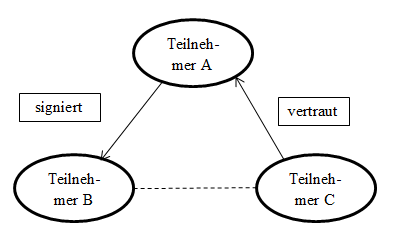
\includegraphics[width=0.4\textwidth]{images/WOT.png}
	\end{center}
	\caption[Web of Trust Vertrauensmodell]{Web of Trust Vertrauensmodell\footnotemark}
	In Anlehnung an: \footcite[S. 120]{Ertel2012}
Teilnehmer C möchte Teilnehmer B eine verschlüsselte Nachricht schicken. Dazu besorgt er sich zunächst das Zertifikat von Teilnehmer B. Dieser wurde zuvor von Teilnehmer A signiert. Da Teilnehmer C Teilnehmer A vertraut, beschafft sich Teilnehmer C den öffentlichen Schlüssel von Teilnehmer A und verifiziert mit damit das Zertifikat von Teilnehmer B. Ist die Verifizierung erfolgreich, so kann Teilnehmer C den öffentlichen Schlüssel von Teilnehmer B vertrauen.

Bei diesem Modell wird zwischen zwei Arten des Vertrauens unterschieden. Einerseits existiert das Vertrauen in eine Person bzw. dessen Signatur. Andererseits besteht ein Vertrauen in einen signierten Schlüssel eines Dritten, der von einer vertrauensvollen Person signiert wurde. Beide Arten des Vertrauens können unabhängig voneinander existieren.